%% USEFUL LINKS:
%% -------------
%%
%% - UiO LaTeX guides:          https://www.mn.uio.no/ifi/tjenester/it/hjelp/latex/
%% - Mathematics:               https://en.wikibooks.org/wiki/LaTeX/Mathematics
%% - Physics:                   https://ctan.uib.no/macros/latex/contrib/physics/physics.pdf
%% - Basics of Tikz:            https://en.wikibooks.org/wiki/LaTeX/PGF/Tikz
%% - All the colors!            https://en.wikibooks.org/wiki/LaTeX/Colors
%% - How to make tables:        https://en.wikibooks.org/wiki/LaTeX/Tables
%% - Code listing styles:       https://en.wikibooks.org/wiki/LaTeX/Source_Code_Listings
%% - \includegraphics           https://en.wikibooks.org/wiki/LaTeX/Importing_Graphics
%% - Learn more about figures:  https://en.wikibooks.org/wiki/LaTeX/Floats,_Figures_and_Captions
%% - Automagic bibliography:    https://en.wikibooks.org/wiki/LaTeX/Bibliography_Management  (this one is kinda difficult the first time)
%%
%%                              (This document is of class "revtex4-1", the REVTeX Guide explains how the class works)
%%   REVTeX Guide:              http://www.physics.csbsju.edu/370/papers/Journal_Style_Manuals/auguide4-1.pdf
%%
%% COMPILING THE .pdf FILE IN THE LINUX IN THE TERMINAL
%% ----------------------------------------------------
%%
%% [terminal]$ pdflatex report_example.tex
%%
%% Run the command twice, always.
%%
%% When using references, footnotes, etc. you should run the following chain of commands:
%%
%% [terminal]$ pdflatex report_example.tex
%% [terminal]$ bibtex report_example
%% [terminal]$ pdflatex report_example.tex
%% [terminal]$ pdflatex report_example.tex
%%
%% This series of commands can of course be gathered into a single-line command:
%% [terminal]$ pdflatex report_example.tex && bibtex report_example.aux && pdflatex report_example.tex && pdflatex report_example.tex
%%
%% ----------------------------------------------------


\documentclass[english,notitlepage,reprint,nofootinbib]{revtex4-1}  % defines the basic parameters of the document
% For preview: skriv i terminal: latexmk -pdf -pvc filnavn
% If you want a single-column, remove "reprint"

% Allows special characters (including æøå)
\usepackage[utf8]{inputenc}
% \usepackage[english]{babel}

%% Note that you may need to download some of these packages manually, it depends on your setup.
%% I recommend downloading TeXMaker, because it includes a large library of the most common packages.

\usepackage{physics,amssymb}  % mathematical symbols (physics imports amsmath)
\include{amsmath}
\usepackage{graphicx}         % include graphics such as plots
\usepackage{xcolor}           % set colors
\usepackage{hyperref}         % automagic cross-referencing
\usepackage{listings}         % display code
\usepackage{subfigure}        % imports a lot of cool and useful figure commands
% \usepackage{float}
%\usepackage[section]{placeins}
\usepackage{algorithm}
\usepackage[noend]{algpseudocode}
\usepackage{subfigure}
\usepackage{tikz}
\usetikzlibrary{quantikz}
% defines the color of hyperref objects
% Blending two colors:  blue!80!black  =  80% blue and 20% black
\hypersetup{ % this is just my personal choice, feel free to change things
    colorlinks,
    linkcolor={red!50!black},
    citecolor={blue!50!black},
    urlcolor={blue!80!black}}


% ===========================================


\begin{document}

\title{Simulation of a penning trap}
\author{Simon Halstensen, Carl Fredrik Nordbø, Herman Brunborg \& Didrik Sten Ingebrigtsen}
\date{\today}
\noaffiliation                            % ignore this, but keep it.

\begin{abstract}
\label{section:abstract}
We have investigated the resonance of particles in an idealized penning trap with a time-dependent electric potential. To accomplish this, we have run penning trap-simulations with $\text{Ca}^{+}$-ions for electric potentials with different frequencies and amplitudes. Through these simulations we find the resonance frequencies of the calcium particles in the penning trap. We proceed to run more simulations with 100 $\text{Ca}^{+}$-ions with coulomb interactions between particles for a resonance frequency. We ultimately find that the particle interactions disrupt the resonance of the $\text{Ca}^{+}$-ions in the penning trap.

\end{abstract}
\maketitle

\section{Introduction}
In this report, we are examining how particles behave in a penning trap. A penning trap is a device that applies a homogenous magnetic field and an inhomogenous electric field in an area to trap a charged particle. The penning trap can be a very useful tool for physicists, which is why we are using numerical simulations to study it.
\\\\
In particular we will look at $\text{Ca}^+$-ions in a penning trap with a time-dependent, periodic electric potential. When applying a time-dependent force to particles, such as the force from our electric field, resonance can occur. We intend to use numerical simulations to find out under what circumstances resonance occurs in the penning trap. More concretely, we will use the algorithm Runge-Kutta 4 to solve the equations of motion of the particles numerically.
\\\\
In the methods-section we will first explain the physics we use in the report. Next, we derive an analytical solution for the movement of a single particle in a penning trap with a constant electric potential, and bounds for solutions where the particles remain in the trap. We wrap up the methods-section by explaining the algorithm Runge-Kutta 4. In the results and discussion-section we first look at the performance of Runge-Kutta 4. Next, we find resonance frequencies of $\text{Ca}^+$-ions by simulating a penning trap with a time-dependent electric potential. We proceed to simulate 100 particles in the penning trap for a resonance frequency, both with and without coulomb interactions between particles. 


\section{Methods}\label{sec:methods}
We model the particles being trapped inside the Penning trap with ordinary differential equations (ODEs) derived from foundational physics equations. Let us quickly go through them here, before using them to argue our model is valid. The first of these equations is Newton's second law (\ref{eq:fun_newton}), which we use to say something about how our particles' velocity is changed in relation to outside forces. Here $m$ is the mass of the particle, while $r$ is its position in Euclidean space. $F_i$ is the $i$th force.
%
\begin{equation}
\label{eq:fun_newton}
m \ddot r = \sum_i F_i
\end{equation}
%
Next comes the equation for how strong an electric field is at a point $r$, when the field is set up by point charges (\ref{eq:fun_couloumb}). In this equation we introduce $k_e$ as Couloumb's constant, $q$ as charge, and say that $q_j$ and $r_j$ are the $j$th particles' charge and position respectively.
%
\begin{equation}
\label{eq:fun_couloumb}
E = k_e \sum_{j=1}^n q_j \frac{r - r_j}{\abs{r - r_j}^3}
\end{equation}
%
Electric fields ($E$) and potential ($V$) are related through (\ref{eq:fun_field_potential}).
\begin{equation}
\label{eq:fun_field_potential}
E = - \nabla V
\end{equation}
%
Lastly, the Lorentz force (\ref{eq:fun_lorentz}) is the force acting on a charged particle moving through an electrical and magnetic field, where the magnetic field is represented by $B$.
%
\begin{equation}
\label{eq:fun_lorentz}
F = qE + qv \times B 
\end{equation}

In addition to these fundamental equations, we have two equations describing how an idealized Penning trap work, that we need to use for our model as well. The electric potential inside the trap is defined by (\ref{eq:potential}), where $V_0$ is the potential applied at the terminals, $d$ is the characteristic distance, a dimensionless size, and $x$, $y$ and $z$ together make up a position.
%
\begin{equation}
\label{eq:potential}
V(x, y, z) = \frac{V_0}{2d^2}(2z^2 - x^2 - y^2)
\end{equation}
%
The magnetic field in the trap is defined as in (\ref{eq:magnetic}). Here, $B_0$ is the field strength.
%
\begin{equation}
\label{eq:magnetic}
B = B_0 \hat{e}_z = (0, 0, B_0)
\end{equation}

With these equations, we can start to model how particles would behave in proximity of or inside the trap. Using (\ref{eq:fun_newton}) and (\ref{eq:fun_lorentz}), and then inserting the properties of our electrical (\ref{eq:potential}) and magnetic (\ref{eq:magnetic}) fields, we get
%
\begin{align*}
m \ddot r &= qE + q\dot r \times B \\
0 &= - m \ddot r + q(- \nabla V) + q\dot r \times B_0 \hat{e}_z \\
0 &= - m \ddot r + q \frac{V_0}{2d^2} \begin{pmatrix} -2x \\ -2y \\ 4z \end{pmatrix}
          + q \begin{pmatrix} \dot y B_0 \\ -\dot x B_0 \\ 0 \end{pmatrix} \\
0 &= \frac{1}{m}
    \begin{pmatrix} 
        \ddot x - q V_0 x / d^2 - q \dot y B_0 \\
        \ddot y - q V_0 y / d^2 + q \dot x B_0 \\
        \ddot z + q V_0 2z / d^2 \\
    \end{pmatrix}
\end{align*}
%
If we now introduce $\omega_0 = \frac{q B_0}{m}$ and $\omega_z^2 = \frac{2qV_0}{md^2}$, and split the vector equations into separate equations, we have that
% Vi burde si noe om tolkningen til omega-variablene, men jeg vet ikke helt hva den er jeg
%
\begin{align}
\label{eq:ode_x} \ddot x - \omega_z^2 x / 2 - \omega_0 \dot y & = 0 \\
\label{eq:ode_y} \ddot y - \omega_z^2 y / 2 + \omega_0 \dot x &= 0 \\
\label{eq:ode_z} \ddot z + \omega_z^2 z &= 0
\end{align}
%
This is a set of three ODEs, where the two first of them are coupled. To solve them more easily, we introduce the complex function $f = x + i y$. Differentiating this twice with regards to time gives us two other equations that we can use to rewrite (\ref{eq:ode_x}) and (\ref{eq:ode_y}) into one complex equation.
%
\begin{equation*}
\dot f = \dot x + i \dot y, \text{ and } \ddot f = \ddot x + i \ddot y.
\end{equation*}
%
We begin with (\ref{eq:ode_x}), and insert expressions for $\ddot x$, $\dot y$ and $x$ derived from our expression for $f$.
%
\begin{align*}
\ddot x - \omega_0 \dot y + \frac{1}{2} \omega_z^2 x &= 0 \\
\left( \ddot f - i \ddot y \right) - \omega_0 \left( \frac{\dot f \dot x}{i} \right) + \frac{1}{2} \omega_z^2 \left( f - iy \right) &= 0
\end{align*}
%
We then insert an expression for $\ddot y$ derived from $f$, and get
%
\begin{align*}
\ddot f - i \left( - \omega_0 \dot x + \frac{1}{2} \omega_z^2 y \right) + i \omega_0 \dot f \dot x + \frac{1}{2} \omega_z^2 \left( f - iy \right) &= 0 \\
\ddot f + i \omega_0 \dot x - \omega_0 \dot x + \frac{1}{2} \omega_z^2 i y - \frac{1}{2} \omega_z^2 i y + i \omega_0 \dot f - \frac{1}{2} \omega_z^2 f &= 0 \\
\ddot f + i \omega_0 \dot f - \frac{1}{2} \omega_z^2 f &= 0
\end{align*}
%
We now have two ODEs that together describe how particles behave in and around our trap. $\ddot f + i \omega_0 \dot f - 1/2 \omega_z^2 f = 0$ gives us information about the $x$-axis ($\Re(f)$) and $y$-axis ($\Im(f)$), and $\ddot z + \omega_z^2 z = 0$ describes the movement along the $z$-axis.

Let us now analyse how our model predicts the particles will behave in the $xy$-plane. The analytical solution of our complex ODE is 
%
\begin{equation}
f(t) = A_+e^{-\omega_+ t} + A_-e^{-\omega_- t},
\label{eq:analytical_solution_xy}
\end{equation}
%
where
\begin{equation*}
\omega_\pm = \frac{\omega_0 \pm \sqrt{\omega_0^2 - 2 \omega_z^2}}{2},
\end{equation*}
and $A_\pm$ are constants set after inserting initial conditions.
%
If we want to trap the particles, we want $\abs{f(t)} < \infty$ even when $t \to \infty$. This means the real component of the exponent must be non-positive, in other words $\text{Re}(-i\omega_\pm) \leq 0$. It could also be that only one of our two terms have non-positive exponents, and $A$ associated with the other term is $0$, but this is highly dependent on initial conditions, and thus very unstable. To understand the relationship between our trap's parameters ($B_0$, $V_0$ and $d$) and the particle's properties ($q$ and $m$), let us expand our $\omega_\pm$-expression and solve the resulting equation.
%
\begin{align*}
0 &\geq \text{Re} \left(-i \omega_\pm \right) \\
  &= \text{Im} \left(- \omega_\pm \right) \\
  &= \frac{1}{2} \text{Im} \left(- \omega_0 \mp \sqrt{\omega_0^2 - 2 \omega_z^2} \right) \\
  &= \text{Im} \left(- \omega_0 \right) + \text{Im} \left( \mp \sqrt{\omega_0^2 - 2 \omega_z^2} \right) \\
  &= \mp \text{Im} \left( \sqrt{\omega_0^2 - 2 \omega_z^2} \right).
\end{align*}
%
This means the imaginary component of the square root must have a strict equality with $0$, which only happens if $\omega_0^2 - 2 \omega_z^2 > 0$, meaning that we get
%
\begin{align*}
\frac{4V_0}{d^2 B_0^2} &< \frac{q}{m},
\end{align*}

if we insert our expressions for $\omega_0$ and $\omega_z^2$. This last equation gives us some opportunity to interpret how the particle should behave. The key insight it provides is perhaps that we have to balance the electrical field with that keeps the particles centered in the $z$-axis with the magnetic field that centers it in the $xy$-plane, because the electrical field also exerts an outwards-pushing force on the particle in the $xy$-plane. It also means that the higher the charge of the particle, and lower mass it has, the higher the potential applied to the terminals can be without it pushing the particle out of the trap in the $xy$-plane.

The fact that the real component of the exponents has to be $0$ also lets us know something about the upper and lower bounds for the distance the particles can have from the origin in the $xy$-plane. Breaking up the motion of the particles in to $f(t) = g(t) + h(t)$, where $g(t) = A_+e^{i\omega_+ t}$ and $h(t) = A_-e^{i\omega_- t}$, we have that $|g(t)| = |A_+|$ and $|h(t)| = |A_-|$ for all $t$. In other words, $g$ and $h$ describe circular motion in the complex plane, with radii $|A_+|$ and $|A_-|$ respectively, and center in the origin. Then the argument for finding upper and lower bounds on the distance to the origin is a simple geometric one. We get the upper bound $R_+$ if $\text{Arg}(g(t)) = \text{Arg}(h(t))$, i.e when $g(t)$ and $h(t)$ contributes in the same direction. Then clearly $|f(t)| = ||A_+| + |A_-||$, meaning $R_+ = |A_+| + |A_-|$. We get our lower bound if $g(t)$ and $h(t)$ contributes in opposite directions. Then $|f(t)| = ||A_+| - |A_-||$, so $R_- = ||A_+| - |A_-||$. % Plot?


%TODO: Regne ut resonansfrekvens:
for $k \in \mathcal{Z}$
$$\Im(-i \omega_\pm \Delta t) = 2 \pi k$$

\section*{The algorithm}
In this project we will be using Runge-Kutta 4 to solve our ODE's on the time-interval $[0, T]$, for n intervals of length h. Runge-Kutta 4 is a fourth order Runge-Kutta method with an error of $\epsilon = \mathcal{O}(h^4)$ . It is a general method for solving ODE's, but here we will adapt the algorithm to solve the equations of motion when an expression $a(r, t)$ for the acceleration is known from \ref{eq:fun_newton}. Assuming that you know the initial position $r_0$ and initial velocity $\dot{r}_0=v_0$ of a particle, we can approximate and discretise the differential equation with Runge-Kutta 4. To numerically solve the equations such that $r_i \approx r(ih)$ and $v_i \approx v(ih)$ for $i \in \{0, 1, 2, \ldots, n\}$, we use algorithm(ref TODO).
%fikk ikke til å sette inn i algorithm-block uten at koden sluttet å kjøre

% TODO: Add these lines for a nicer plot
\begin{algorithm}
\caption{An algorithm with caption}\label{alg:cap} % TODO: Name the code box
\begin{algorithmic}[1]
\State $r_0 \gets r(0)$
    \State $v_0 \gets v(0)$
    \State $n \gets \dfrac{T}{h}$
    \For{$i \in \{1, 2, \ldots, n\}$}
        \State $K_{1,v} \gets a(r_i, t_i)$
        \State $K_{1,r} \gets v_i$
        \State $K_{2,v} \gets a(r_i + \dfrac{h}{2}K_{1,v}, t_i + \dfrac{h}{2})$
        \State $K_{2,r} \gets v_i + \dfrac{h}{2} K_{1,r}$
        \State $K_{3,v} \gets a(r_i + \dfrac{h}{2}K_{2,v}, t_i + \dfrac{h}{2})$
        \State $K_{3,r} \gets v_i + \dfrac{h}{2} K_{2,v}$
        \State $K_{4, v} \gets a(r_i + hK_{3,v}, t_i+h)$
        \State $K_{4, r} \gets v_i + hK_{3,r}$
        \State $v_i = \dfrac{h}{6}(K_{1,v} + 2K_{2,v} + 2K_{3,v} + K_{4,v})$
        \State $r_i = \dfrac{h}{6}(K_{1,r} + 2K_{2,r} + 2K_{3,r} + K_{4,r})$
    \EndFor
    \Return{$v, r$}
\end{algorithmic}
\end{algorithm}

In reality, the code may be slightly more complex than what is found in the (REF) as multiple particles are able to interact with each other.
%%% ------------------------------------------------------------------------ %%%
% Har bare ført inn en introduksjon til problem 4, men tror problem 1-3 er helt 
% ok ført nå. I problem 4 husker jeg ikke og klarer ikke finne en forklaring på
% del 2, men del 1 har jeg kontroll på.
% Det er litt mange ligninger og mye matte per forklaring, men det er mulig det 
% er vanskelig å unngå. Kan hende vi kan slippe unna med mindre mellomregning 
% da.
%%% ------------------------------------------------------------------------ %%%



\section{Results and discussion}\label{sec:results}
\begin{figure}[h]
    \centering
    \text{Simulation of particle position for $p_0=(100, 0, 100)$,}
    \text{$v_0=(0, 1, 0)$, $\Delta t=10^{-3}$, $N=10^5$}
    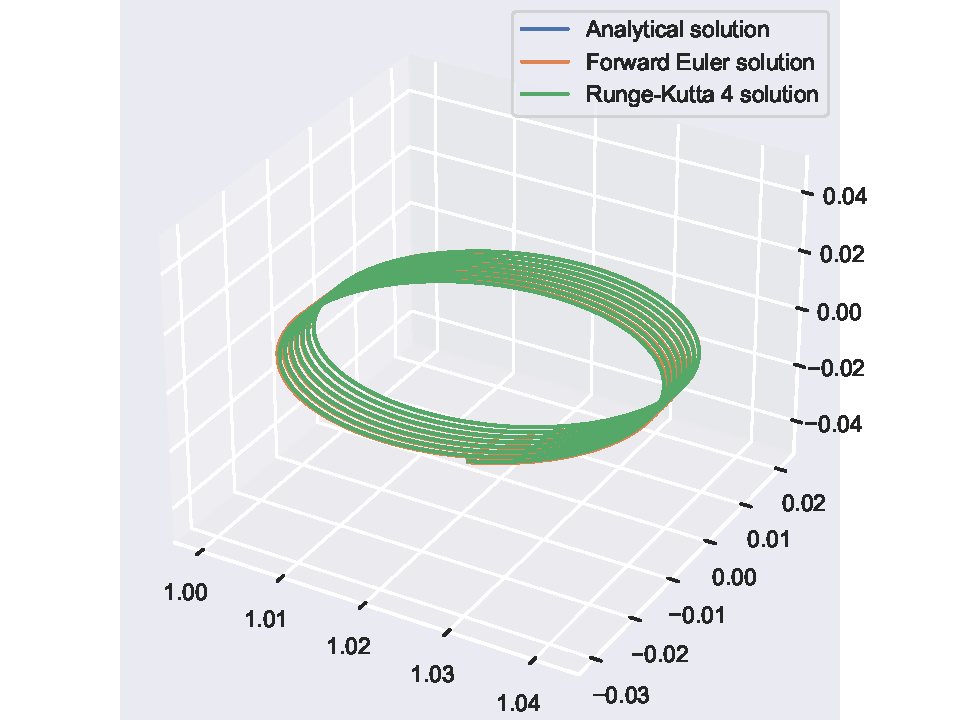
\includegraphics[width=0.5\textwidth]{data/position_estimates.pdf}
    \caption{The position of the particle as according to the analytical solution, a Forward Euler simulation and a Runge-Kutta 4 simulation}
    \label{fig:estimated_positions}
\end{figure}

Simulating the penning trap with Runge-Kutta 4 gives output that follows the analytical solution very closely. In comparison we observe some very small deviation in the solution from Forward Euler (FIG. \ref{fig:estimated_positions}). 
\\\\
Figure (\ref{fig:runge_kutta_relative_error}) more closely analyzes the error of our simulation. Here we show the relative error using 5 different step sizes and $t \in [0, 100]\mu s$. In figure (\ref{fig:forward_euler_relative_error}) we do the same for Forward Euler. Using this we get to say something about the rate of convergence for Runge-Kutta 4 and Forward Euler. For Forward Euler we estimate $r_\text{err} = 0.811$, while Runge-Kutta 4 as expected performs better at $r_\text{err} = 1.93$. While this is significantly lower than the expected $\mathcal{O}(h^4)$, this might be because this is a poor estimate. This might have something to do with the anomalies we see in figure (\ref{fig:runge_kutta_relative_error}).
\\\\
We clearly see from our results that the step size affect the precision of the simulation, with smaller step sizes giving solutions closer to the analytic one. When deciding on a step size for finding resonance, precision is obviously a concern. However smaller step sizes also gives more computationally heavy simulations. With this in mind, we decided on a step size of $h=10^{-2}$.
\\\\
It's also worth noting that the error grows as $t$ grows. This is important as we are about to look at the state of the penning trap 500$\mu s$ in.
\\\\
Figure (\ref{fig:two_particles_xy_plane}) shows the effect of turning off the coulomb interactions, as a plot of the path in the xy-plane. Figure (\ref{fig:two_particles_xy_plane_3d}) also shows the effect of turning off the interactions, with a 3D-plot of the trajectories of the particles. As expected, turning off coulomb interactions slightly alters the path of the particle. Importantly, turning off coulomb interactions greatly reduces the time it takes to carry out the simulations. This means we can simulate many more particles, as we need to when looking for resonance.
\\\\
\begin{figure}[h]
    \centering
     \text{Relative error of Runge Kutta 4}
    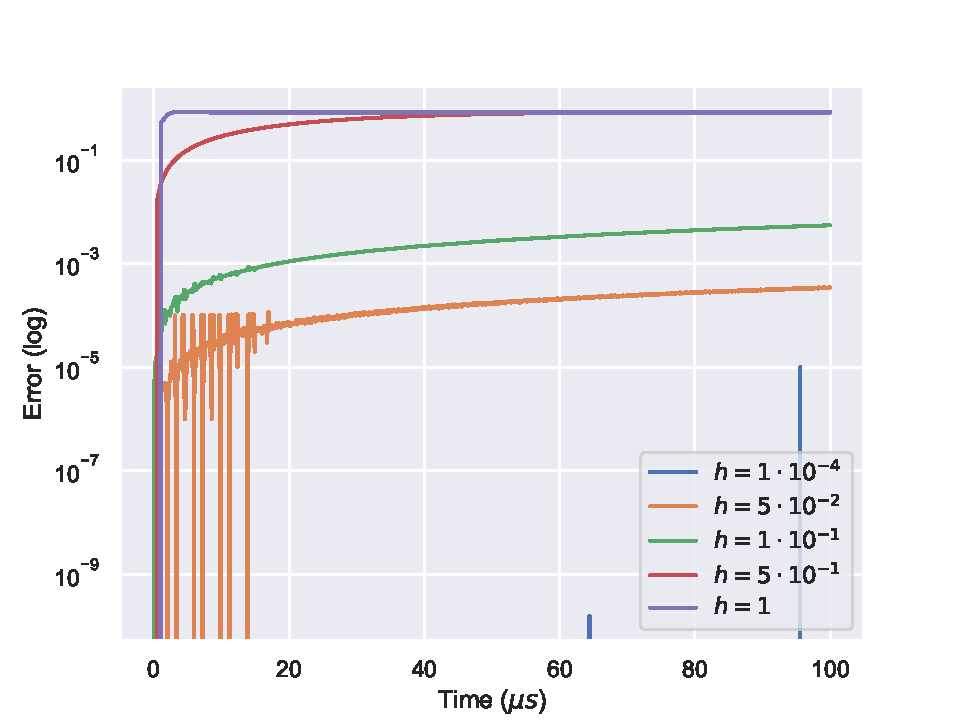
\includegraphics[width=0.5\textwidth]{data/runge_kutta_4_relativeError.pdf}
    \caption{The relative error for the Runge-Kutta 4 method as compared to the analytical solution}
    \label{fig:runge_kutta_relative_error}
\end{figure}
\begin{figure}[h]
    \centering
    \text{Relative error of Forward Euler}
    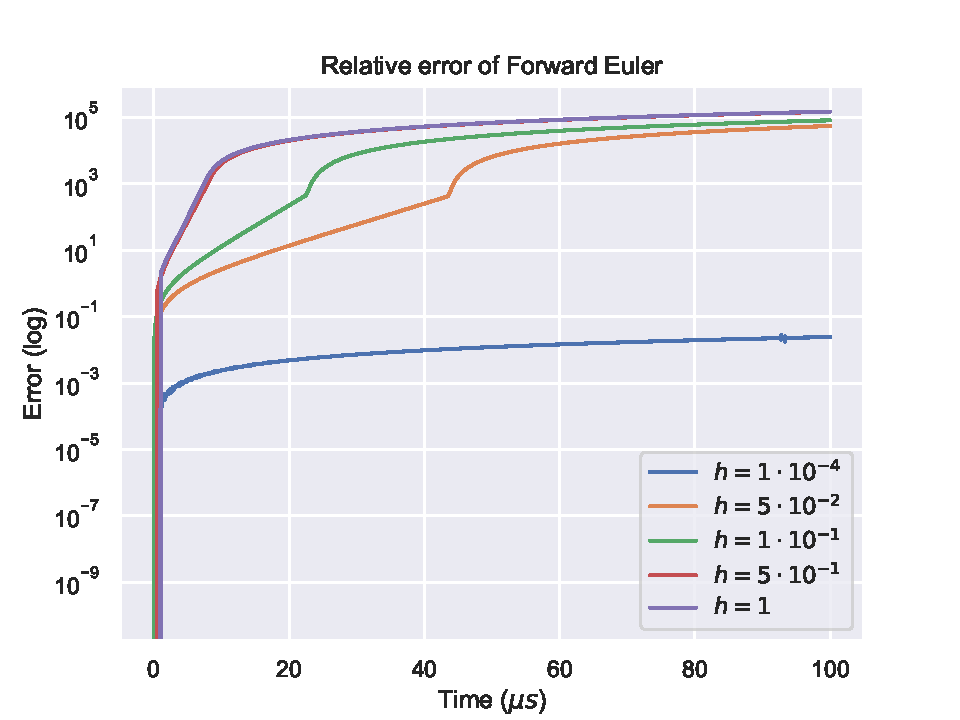
\includegraphics[width=0.5\textwidth]{data/forward_euler_relativeError.pdf}
    \caption{The relative error for the Forward Euler method as compared to the analytical solution}
    \label{fig:forward_euler_relative_error}
\end{figure}
% TODO: Place the correct place
\begin{figure}[h]
    \centering
    \text{Motion of two particles in the xy-plane}
    \text{with and without coulomb interaction}
    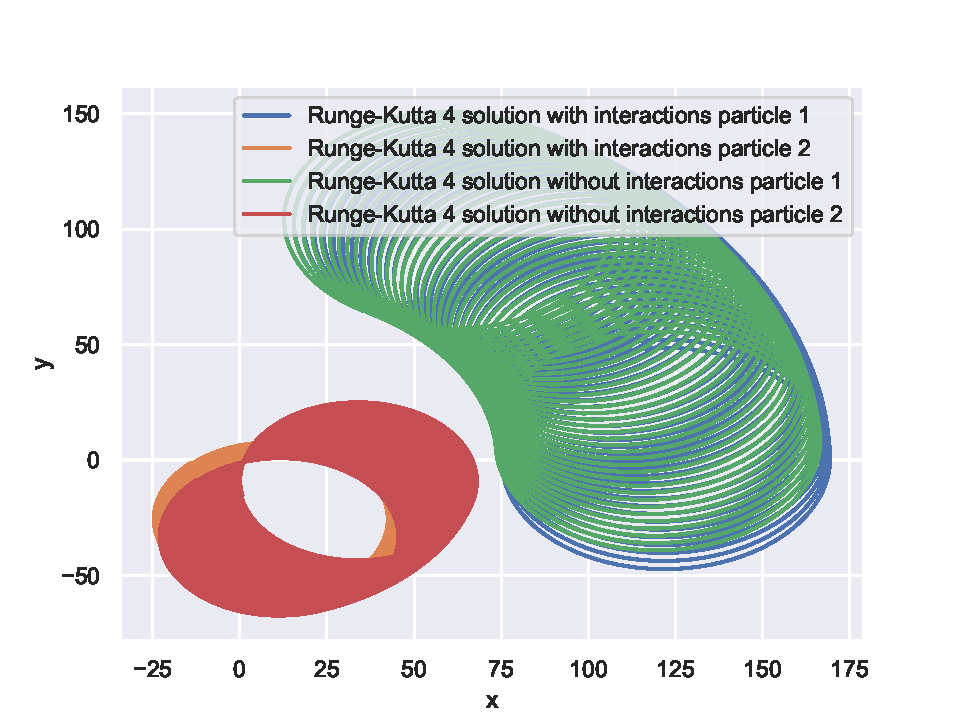
\includegraphics[width=0.5\textwidth]{data/two_particles_2d.pdf}
    \caption{The simulations of two particles with and without coulomb interactions}
    \label{fig:two_particles_xy_plane}
\end{figure}
\begin{figure}[h]
    \centering
    \text{Motion of two particles in the xy-plane}
    \text{with and without interaction in 3D}
    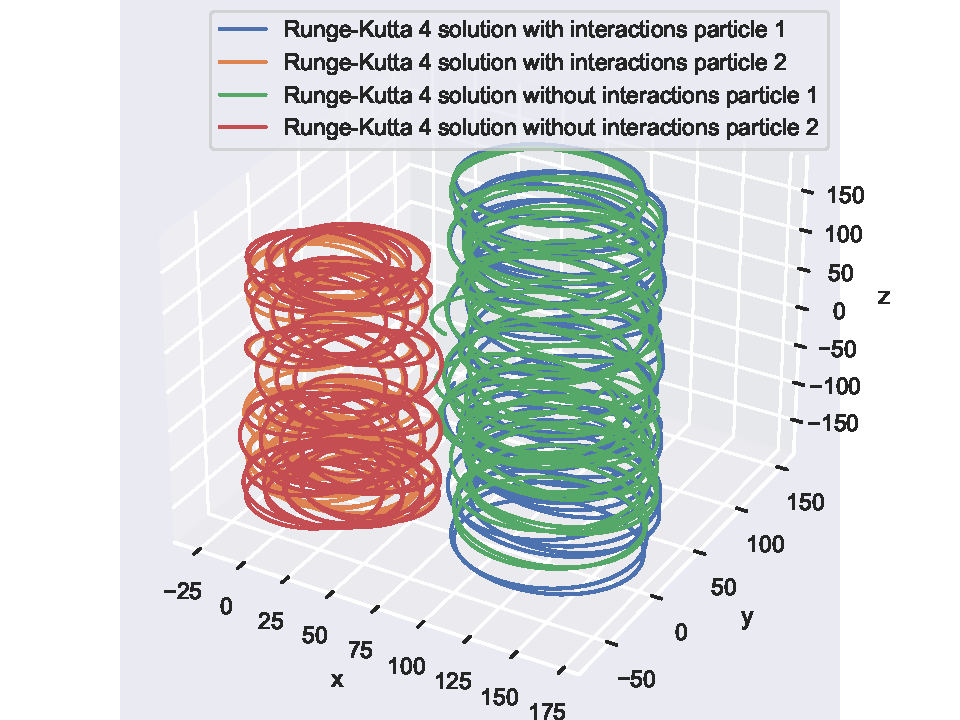
\includegraphics[width=0.5\textwidth]{data/two_particles_3d.pdf}
    \caption{The simulations of two particles with and without coulomb interactions in 3d}
    \label{fig:two_particles_xy_plane_3d}
\end{figure}

\begin{figure}[h]
    \centering
    \text{Particles left after $500$ $\mu s$}
    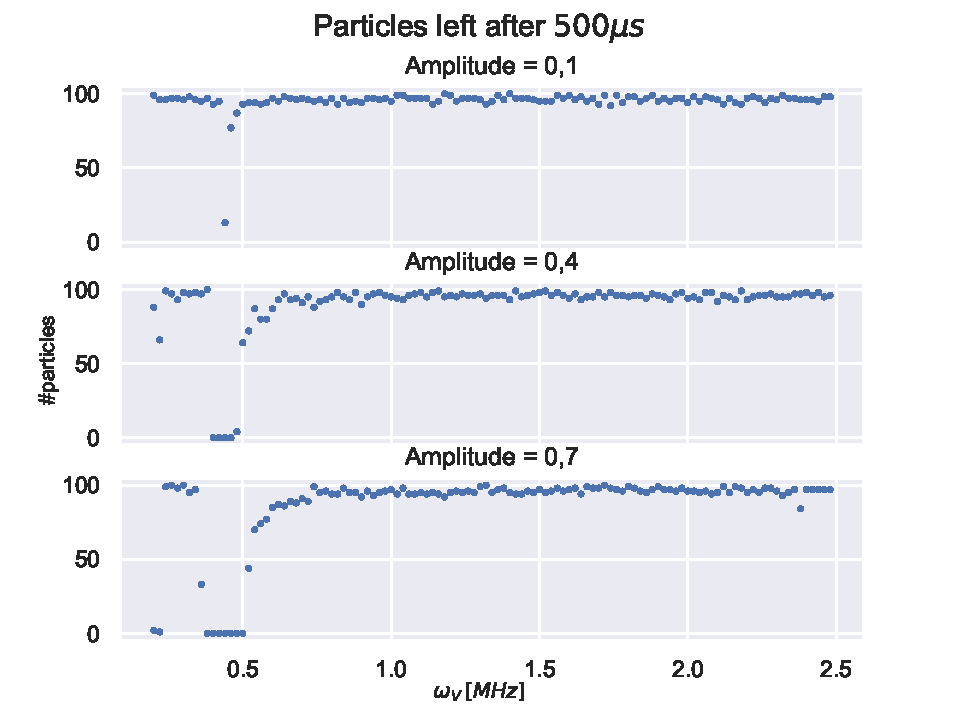
\includegraphics[width=0.5\textwidth]{data/particles_left_rough_grained.pdf}
    \caption{Particles left in the penning trap for different frequencies}
    \label{fig:particles_left_rough_grained}
\end{figure}
\begin{figure}[h]
    \centering
    \text{Particles left after $500$ $\mu s$}
    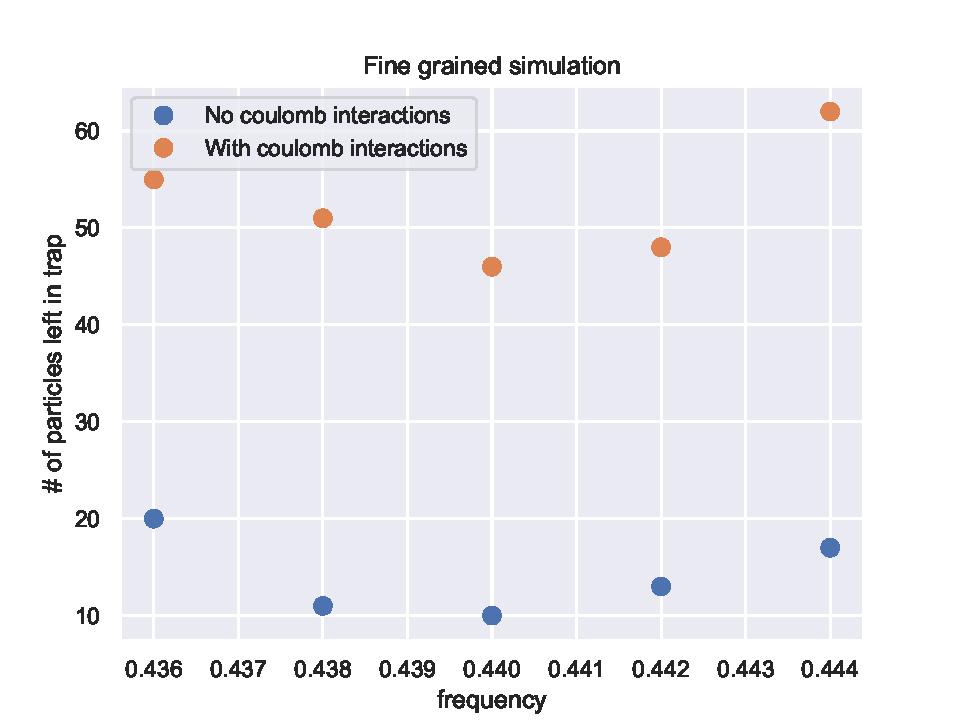
\includegraphics[width=0.5\textwidth]{data/particles_left_fine_grained.pdf}
    \caption{Particles left in the penning trap for different frequencies with and w/o coulomb interactions}
    \label{fig:particles_left_fine_grained}
\end{figure}

For a time-dependent electric field we repeated simulations of 100 $\text{Ca}^{+}$-ions with amplitudes $f = 0.1, 0.4, 0.7$, without coulomb interactions. We did the simulations for evenly spaced frequencies $\omega_V$ in the interval $[0.2, 2.5]\text{MHz}$, and counted the number of particles left in the penning trap after $500\mu s$ for a step size $h=10^{-2}$. Figure (\ref{fig:particles_left_rough_grained}) shows that for all of the amplitudes tested there is a significant lowering of the number of particles left in the trap when the frequency is $\omega_V \approx 0.44 \text{MHz}$. We also can see a clear lowering of particles left for $\omega_V \approx 0.22 \text{MHz}$ for $f=0.7$. 
\\\\
The fact that the resonance frequency at $0.22$ is half of the resonance frequency $0.44$ is a reasonable result. In general if $\omega_{V,0}$ is the fundamental frequency, the highest resonance frequency, then $\dfrac{\omega_{V,0}}{2}, \dfrac{\omega_{V,0}}{3}, \dfrac{\omega_{V,0}}{4} \ldots$ are all resonance frequencies\cite{harmonic}. In our case, $0.44$ appears to be our fundamental frequency, which fits with our finding that $\dfrac{0.44}{2}$ is also a resonance frequency.
\\\\
As the external electric force is a periodic, time-dependent force, it is natural to explain the behavior of the particles with resonance. If a calcium ion has a resonance frequency equal to the frequency $\omega_V$ of the electric field, the oscillation of the particle is amplified. This is seemingly what is happening in our simulations. If the frequency of the electric field is close to a resonance frequency of the calcium ions, the particles' oscillations increase in amplitude. This can in turn lead to the particles moving outside of the penning trap, which is why certain frequencies $\omega_V$ lead to a large amount of particles leaving the trap.
\\\\
We can also see that the breadth of the interval of frequencies where the particles all leave the trap increases as the magnitude of the electric field oscillation increases. As the magnitude increases, the oscillations become bigger.
\\\\
Next, we proceeded to do a more fine-grained simulation for $f=0.1$, both with and without coulomb interactions around $\omega_V = 0.44 \text{MHz}$. We tested with 5 evenly spaced values of $\omega_V$ in the interval $[0.436, 0.444]\text{MHz}$. As figure (\ref{fig:particles_left_fine_grained}) shows, it seems we have a local minimum for the numbers of particles left after 500$\mu s$ at around $0.44\text{MHz}$. 
\\\\
From figure (\ref{fig:particles_left_fine_grained}) it also seems we observe less resonance when accounting for the interactions between particles. This suggests that the particles' interactions disrupt the resonant oscillation that we observed without particle interactions. This result seems reasonable, as resonance occurs when a periodic force coincides with periodic movement. When coulomb interactions with 99 other particles unpredictably affects the movement of a particle, the movement is no longer perfectly periodic. Therefore it makes sense that there occurs less resonance. 


\section{Conclusion}\label{sec:conclusion}
The first part of the results suggests that we can trust our implementation of Runge-Kutta 4, but that the hardware limitations we are working with might have meant that the results weren't as accurate as they needed to be. We analyzed the system a full $500 \mu s$ in, which meant we would need a very accurate simulation to be able to trust the result at the end.
\\\\
We are nevertheless satisfied with having observed resonance in our penning trap, and having found how the amplitude of the time-dependent potential interacts with this. Also seeing that accounting for coulomb interactions disrupts the resonance phenomena was interesting. 
\\\\
We have some suggestions for further work that could give additional insight into resonance phenomena inside idealized penning traps. In particular, it could be informative to further investigate the conditions that allow us to observe resonance in the penning trap. One could for instance repeat simulations with different amounts of particles to describe the relation between the number of particles and resonance. One could also run fine-grained scans, for frequencies $\omega_V = \dfrac{0.44}{2}, \dfrac{0.44}{3}, \dfrac{0.44}{4}, \ldots$ to check that these are resonance frequencies.
\\\\
Additionally, we would want to optimize and parallelize the source code, so we could realistically run the simulations with a smaller step size. 


\section{Appendix \romannumeral 1}\label{sec:appendixI}
To test our implementation, we want to find a specific analytical solution given some initial conditions, and compare this with what our numerical approach gives us. Let us therefore assume we have a single charges particle in our Penning trap, with
%
\begin{align*}
x(0) = x_0, \quad \dot x(0) = 0, &\quad y(0) = 0, \quad \dot y(0) = v_0, \\
z(0) = z_0, \text{ an}&\text{d} \quad \dot z(0) = 0.
\end{align*}
%
Next, we find the general analytical solution for the $z$-axis by rewriting (\ref{eq:ode_z}) as two first order differential equations
%
\begin{align}
\dot z_0 = z_1, \text{ and } \dot z_1 = - \omega_z^2 z_0
\label{eq:ode_z_coupled}
\end{align}
%
where $z_0 = z$, and $z_1 = \dot z$. 


\onecolumngrid

%\bibliographystyle{apalike}
\bibliography{ref}


\end{document}
